\section{Method: Survey}\label{section:Method_survey}
The validity of the the Prototype was tested using a survey.
If a survey is not well designed then it could lead to invalid or irrelevant outcomes.
As well as describing the design and procedure of the survey, we also outline any threats to its validity in this chapter.
Our choice of survey technique is a Questionnaire.

\subsection{Questionnaire Design}
The questionnaire can be found in appendix \ref{Appendix:Questionaire_text}.
To design the survey of our prototype, we followed a number of rules derived from the works of Bryman\cite{bryman2016social} and de Vaus\cite{de2013surveys}.

As advised, first we devised a clear introduction to describe the research.

We considered existing questions.
With regards to projectional editing, we requested the original questionnaires from three papers\cite{meacham2020adaptivevle,berger2016efficiency, voelter2014towards} pertaining to tools developed using projectional editing.
From these questionnaires we found [X] that we considered and decided against using any of them.

When formulating the questions we had the specific research question ``Which projections can help developers to get appropriate feedback about rules?'' in mind.

The pool of Drools users that we were personally in contact with was incredibly small.
Thus we had to rely on responses from strangers.
For this reason, we tried to make the questionnaire as quick to finish as possible.
This meant we looked particularly hard at removing questions that did not help us to our research goal.

We piloted the questionnaire with both ourselves and our industrial supervisor.

The instructions to each of the questions were tested for clarity, by a non-technical third party.

The only open question was one for which we wished to extract sentiment.
Rather than having yes/no questions, where appropriate we applied a Likert scale\cite{likert1932technique}.

The design of survey monkey layout makes sure that questions do not span pages.

The socio-demographic questions (skill level and experience) were left to the end and research based questions were toward at the beginning.

We took care to rework questions that were long, ambiguous, general, or leading to not be so.
We also took care to remove jargon, negative wording, and questions that asked about more than one thing.

\subsection{Participants}

The requirement for participants is that they have at least a little experience with using Drools.
It was our hope to get a statistically significant number of participants.

\subsection{Validity}
Non-response bias\cite{armstrong1977estimating} will be addressed by making the questionnaire short and easy to answer.
Because of the nature of the participant selection for this survey, it will be difficult to address the bias of self selection caused by voluntary response.

Common method bias, i.e. ``variance that is attributable to the measurement method rather than to the construct the measures represent''\cite{podsakoff2003common} can be responsible for 25\% or more of variable relational influence.
As we are only conducting a single survey, we won't be able to do much to prevent this, however we will take the following small precautions.
Testing the survey to remove question ambiguity, mood influences, and length issues.
Mixing the survey order of questions will be used to mitigate the issues caused by similarity of items, proximity of items, and location of items.
We will mitigate survey administration biases by administering some of these questionnaires manually and some online.
We will make sure that there are no right or wrong answers and aim toward fact based questions.
We will vary the scales of our Likert scales and the types of questions.

The main statistical methods to address this bias, i.e. ``Harman's single factor test''\cite{podsakoff2003common} and the``marker variable''\cite{lindell2001accounting} were found to be lacking in grounding\cite{gorrell2011countering}.
Marker variable is considered appropriate if used with caution.
With the size of our expected returns, it may not be possible to gain a statistically significant outcome.

\subsection{Pre-test}
The first attempt at the survey was sent to our industrial supervisor, who has experience with Drools.
We used this to remove ambiguously worded or leading questions and test that the length was truly between 5-10 minutes.
This lead to the following changes:
[TODO: add changes after we have tested]


\subsection{Sampling}
As within our own professional network we only had acquaintance with (6?) Drools developers, we had to expand our reach to those we did not personally know.

Our approach was first search StackOverflow for question askers and answerers on the subject of Drools.
Our preference was to find email addresses, failing that twitter contacts.
This proved to be quite limited, especially in attempting to get contact details, 13 email addresses and 6 twitter addresses.

Our next approach was to trawl our LinkedIn connections for anyone with drools as a proclaimed skill.
Whilst we had no one in our direct contacts, at one level of separation we found 204 connections.
From these we could extract 54 email addresses and 40 twitter addresses, with only a small crossover with the addresses harvested from StackOverflow.

We chose not to expand to third level contacts, as we thought this would be harder to sell as to why they should feel comfortable answering us.

\subsection{Procedure}

The questions, as described in appendix \ref{Appendix:Questionaire_text}, was uploaded to Survey monkey.

To encourage response, especially amongst only tangentially known participants, we crafted a short introduction, using techniques designed to enhance response as discussed by amongst others Cialdini\cite{goldstein2008yes}.
As seen in figure \ref{fig:persuasive_introduction}, the attics discussed by Cialdini, as signposted in table \ref{table:persuasive_introduction}.
\begin{table}[h]
    \begin{center}
        \begin{tabular}{ |l | l |  } 
            \hline
            Key &  Tactic\\
            \hline
            1  & Short option for those with no time \\
            2  & Credentials matter \\
            3  & Recognition, (this might backfire as I hardly remember any of my LinkedIn connections) \\
            4  & Consistency, they reported they have Drools experience, so they must live up to it \\
            5a\&b  & Social Proof - other people have already answered \\
            6  & showing value \\
            7  & Special because of scarcity \\
            8  & Labelling - ``I see you to be a good person'' \\
            9  & The word ``Because'' has an outweighed effect \\
            10 & Compliment Expertise \\
            11 & ``Every little helps'' \\
            12 & point out a fault \\
            13 & own the fault \\
            14 & ask a favour \\
            15 & add inconvenience \\
            16 & Rhyming \\
            17 & hand written note \\
            \hline
        \end{tabular}
    \end{center}
    \caption{Persuasion tactics in figure \ref{fig:persuasive_introduction}}
    \label{table:persuasive_introduction}
\end{table}

\begin{figure}[h]
    \centering
    \fbox{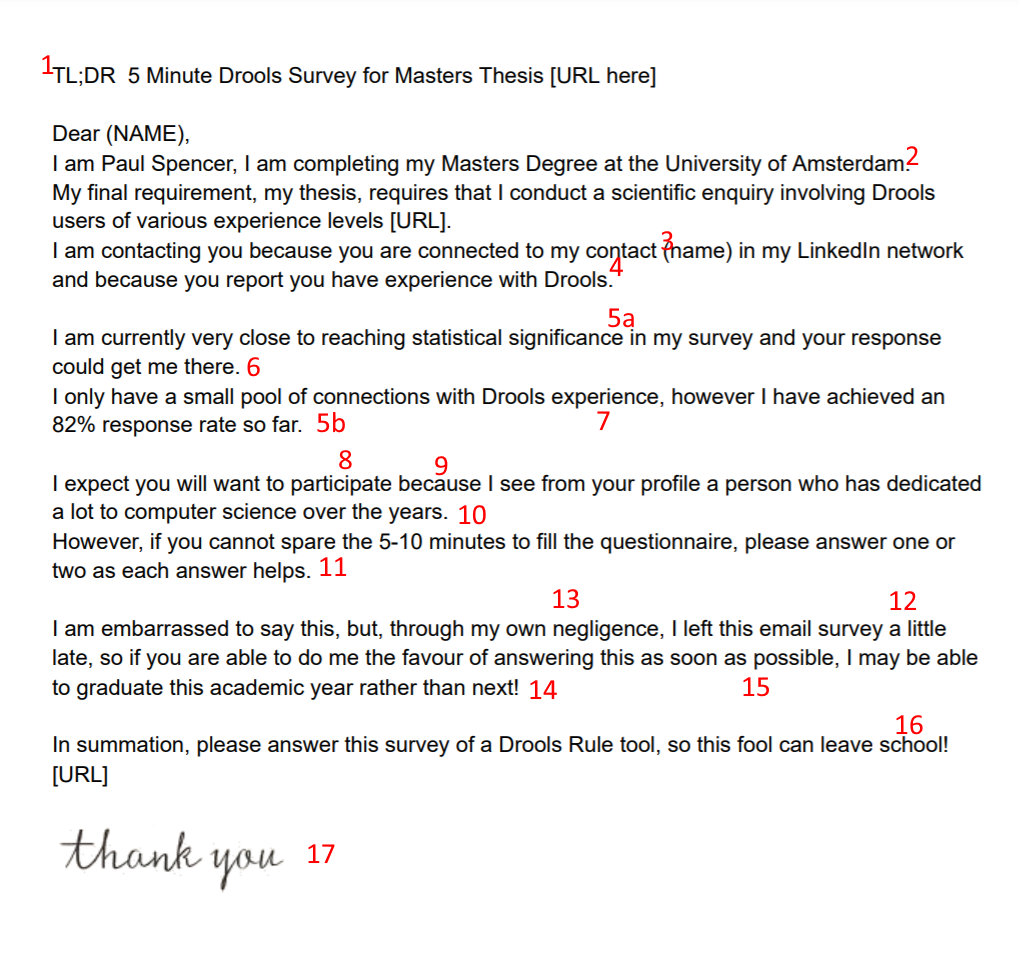
\includegraphics[width=0.85\textwidth]{Sections/images/persuasion.png}}
    \caption{Persuasive introduction}
    \label{fig:persuasive_introduction}
\end{figure}

These were sent to our list of drools using strangers and we sat back and awaited response.
